\chapter{Instrukcja użytkowania biblioteki}

Do pracy dołączona jest biblioteka, zawierająca implementacje omawianych algorytmów, jak również dodatkowe pliki umożliwiające odtworzenie przeprowadzonych eksperymentów. Kod został przetestowany na systemie Windows 11, z zainstalowanym językiem \texttt{Julia}\cite{Julia} w wersji \texttt{1.10.2}. Dodatkowo, do stworzenia wykresów wykorzystano język \texttt{Python}\cite{Python} w wersji \texttt{3.11.9}.  

\subsection*{Struktura plików}

Część implementacyjna pracy zawarta jest w folderze \texttt{src}. Jego strukturę ukazuje rysunek\ref{fig:folder_structure}. Znajdują się w nim dwa główne foldery. Pierwszy z nich, \texttt{chart\_generation} zawiera pliki \texttt{.ipynb} używane do rysowania wykresów na podstawie plików \texttt{.csv}. Drugi folder, \texttt{sketching} zawiera kod właściwej biblioteki. W jej skład wchodzą następujące pliki:
\begin{itemize}
    \item \texttt{DataGenerator.jl} -- zawiera kod do generowania losowych macierzy sąsiedztwa w różnych modelach.
    \item \texttt{DataManager.jl} -- znajdujące się w nim metody pozwalają na wczytywanie i zapisywanie macierzy do plików \texttt{.mat}.
    \item \texttt{ExperimentsSimilarity.jl} -- plik ten zawiera kod umożliwiający testowanie precyzji rekonstrukcji grafów.
    \item \texttt{ExpSketch.jl} -- zawiera implementacje algorytmów \texttt{ExpSketch} i \texttt{FastExpSketch}.
    \item \texttt{Logger.jl} -- pozwala na sterowaniem tym, w jaki sposób wypisywane są informacje na temat działania algorytmów.
    \item \texttt{main\_sim.jl} -- plik ten uruchamia wszystkie eksperymenty związane z badaniem precyzji rekonstrukcji grafu.
    \item \texttt{NodeSketch.jl} -- znajduje się w nim właściwa implementacja algorytmów \texttt{NodeSketch} i \texttt{EdgeSketch}.
    \item \texttt{performance\_testing.jl} -- kod eksperymentu sprawdzającego czas działania algorytmów.
\end{itemize}

\newpage

\begin{figure}[!ht]
    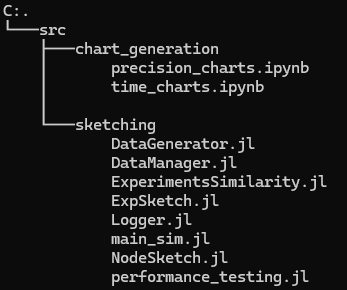
\includegraphics[width=8cm]{img/folder_structure.png}
    \centering
    \caption[Struktura plików]{Struktura plików biblioteki.}
    \label{fig:folder_structure}
\end{figure}

\subsection*{Przykład użycia}

Poniżej przedstawiono przykładowe użycie biblioteki. Wszystkie polecenia zostały w tym przypadku wykonane w interaktywnej konsoli języka \texttt{Julia}. Pierwszym krokiem jest wczytanie pliku \texttt{DataGenerator.jl}, i wygenerowanie grafu w modelu Erdosa-Renyiego o $6$ wierzchołkach, prawdopodobieństwie krawędzi $p = 0.5$ oraz maksymalną wagą krawędzi równą~$1$.

\begin{lstlisting}[basicstyle=\footnotesize]
    julia> include("DataGenerator.jl")
    generate_all (generic function with 1 method)
    
    julia> matrix = generate_erdos_renyi_matrix(6, 0.5, 1)
    6x6 Matrix{Float64}:
     0.0  0.0  0.0  0.0  1.0  0.0
     0.0  0.0  1.0  0.0  1.0  1.0
     0.0  1.0  0.0  1.0  1.0  1.0
     0.0  0.0  1.0  0.0  1.0  0.0
     1.0  1.0  1.0  1.0  0.0  1.0
     0.0  1.0  1.0  0.0  1.0  0.0
\end{lstlisting}

Następnie należy wczytać plik \texttt{NodeSketch.jl}. Poniżej ukazano także wywołanie algorytmu \texttt{NodeSketch} dla wygenerowanej macierzy, z parametrami $k = 2$, $m = 4$ oraz $\alpha = 0.3$.

\begin{lstlisting}[basicstyle=\footnotesize]
    julia> include("NodeSketch.jl")
    Main.NodeSketch
    
    julia> NodeSketch.nodesketch(matrix, 2, 4, 0.3)
    Main.NodeSketch.Sketch([5.0 2.0 ... 2.0 2.0; 5.0 6.0 ... 6.0 6.0; 5.0 2.0 ... 2.0 2.0; 1.0 6.0 ... 1.0 6.0], [1.0 0.0 ... 0.25 0.0; 0.0 1.0 ... 0.75 1.0; ... ; 0.25 0.75 ... 1.0 0.75; 0.0 1.0 ... 0.75 1.0], 96)
\end{lstlisting}

Kolejny przykład ilustruje wywołanie algorytmu \texttt{EdgeSketch} z tymi samymi parametrami. Zwraca on obiekt zawierający trzy pola: \texttt{embeddings} -- macierz zanurzeń wierzchołków, \texttt{similarity\_matrix} -- macierz podobieństwa wierzchołków oraz \texttt{calculated\_hashes}, czyli liczbę obliczonych wartości funkcji haszującej. 

\begin{lstlisting}[basicstyle=\footnotesize]
    julia> res = NodeSketch.edgesketch(matrix, 2, 4, 0.3)
    Main.NodeSketch.Sketch([0.023946932553343094 0.11321003816732249 ... 0.023946932553343094 0.8068069829529673; 0.20572686024856923 0.16361792227247998 ... 0.20572686024856923 0.16361792227247998; 0.2101007056250945 0.0060560405326058765 ... 0.0060560405326058765 1.4828069059435225; 0.10337951871171033 0.32929093744654353 ... 0.08786964958953339 0.3704157329572328], [1.0 0.0 ... 0.5 0.0; 0.0 1.0 ... 0.25 0.25; ... ; 0.5 0.25 ... 1.0 0.0; 0.0 0.25 ... 0.0 1.0], 85)

    julia> res.embeddings
    4x6 Matrix{Float64}:
     0.0239469  0.11321     0.103898    0.238676    0.0239469   0.806807
     0.205727   0.163618    0.957174    0.34143     0.205727    0.163618
     0.210101   0.00605604  0.145416    0.177179    0.00605604  1.48281
     0.10338    0.329291    0.00293567  0.00293567  0.0878696   0.370416
\end{lstlisting}
    